This document describes \emph{AGIOS}\footnote{The tool's name - AGIOS - comes from ``Application-Guided I/O Scheduler'' and is Greek for ``holy''.}. 

\textbf{(If you already know AGIOS and/or are in a hurry, you can skip this introduction and some chapters. Please read this document in this order: Chapter~\ref{chapter:starting}, \ref{chapter:serra}, \ref{chapter:configfile}, and then Chapter~\ref{chapter:citing}.)}

The main objectives for AGIOS' development were to make it generic, non-invasive, easy to use, and to offer multiple choices on scheduling algorithms.

We wanted to develop a tool that could be used by \emph{any I/O service that treats requests at a file level}, such as a local file system or intermediate nodes in an I/O forwarding scheme. For this reason, AGIOS has a library implementation suitable for inclusion on most of today's parallel file systems' servers. On the other hand, AGIOS also offers a kernel module implementation that can be used, for instance, at the virtual file system layer. The I/O services that use AGIOS are called its ``users''. Our AGIOS implementation is deeply inspired by the aIOLi framework\footnote{\url{http://aioli.imag.fr/}}.

\begin{figure}[!h]
\centering
\begin{subfigure}{0.4\textwidth}
\centering
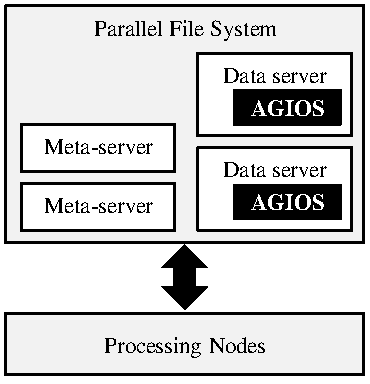
\includegraphics[width=\textwidth]{images/agios_usage_example_1.pdf}
\caption{in a parallel file system's data servers}
\label{fig:agios_usage_example_1}
\end{subfigure}
\hspace{1cm}
\begin{subfigure}{0.4\textwidth}
\centering
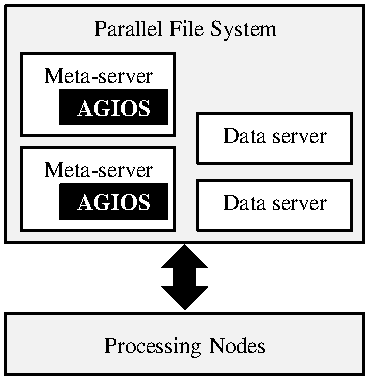
\includegraphics[width=\textwidth]{images/agios_usage_example_2.pdf}
\caption{in a parallel file system's metadata servers}
\end{subfigure}
%\vspace{1cm}
\begin{subfigure}{0.4\textwidth}
\centering
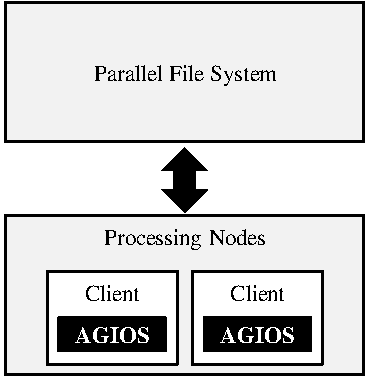
\includegraphics[width=\textwidth]{images/agios_usage_example_3.pdf}
\caption{in the processing nodes (either local VFS or PFS client)}
\end{subfigure}
\hspace{1cm}
\begin{subfigure}{0.4\textwidth}
\centering
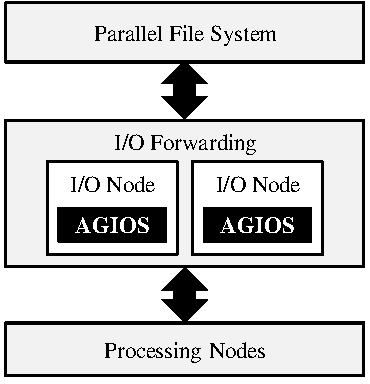
\includegraphics[width=\textwidth]{images/agios_usage_example_4.pdf}
\caption{in the intermediate nodes from an I/O forwarding scheme}
\end{subfigure}
\caption{Four examples of use for AGIOS.} \label{fig:agios_usage_examples}
\end{figure}

Figure~\ref{fig:agios_usage_examples} presents four non exhaustive examples of use for AGIOS. All of the four presented placement options are I/O services that treat requests at a file level, and are places where it makes sense to use I/O scheduling. These placement options are not exclusive, in the sense that we could have all of them happening at the same time. In order to avoid creating a bottleneck, AGIOS instances (on different PFS servers, or at different levels of the I/O stack) are independent and do not make global decisions. 

AGIOS exports a simple interface composed of four steps:

\begin{itemize}

  \item \textbf{Initialization:} The user calls \emph{agios\_init} in order to initialize the AGIOS infrastructure. At this moment, the user must provide a callback function used to process a single request. If a function capable of processing a list of requests at once is available, the user should also provide it.

  \item \textbf{A new request arrives:} The user calls \emph{agios\_add\_request} to transmit the request to the scheduler.

  \item \textbf{Requests are ready to be processed:} The scheduler passes the requests back to its user through the provided callback function. Therefore, the task of processing requests is left to the I/O services using the library.
    This keeps AGIOS' interface simple and generic.

  \item \textbf{Finalization:} The user calls \emph{agios\_exit} for cleaning up the tool's infrastructure.

\end{itemize}

\begin{figure}[h]
\centering
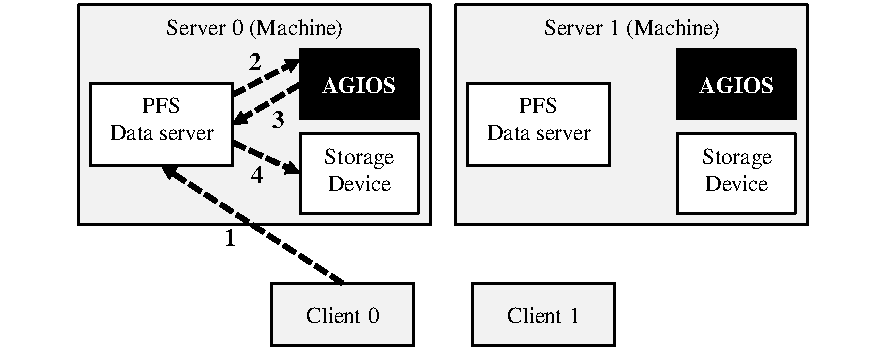
\includegraphics[width=\columnwidth]{images/agios_interface.pdf}
\caption{A request's path to a PFS server with AGIOS.} \label{fig:agios_interface}
\end{figure}

Additional calls are provided to generate access statistics files and to reset statistics.
An illustration of this interface is provided in Figure~\ref{fig:agios_interface}, that shows a situation where AGIOS is used by a parallel file system's data servers (scenario illustrated at Figure~\ref{fig:agios_usage_example_1}). In step \textbf{1}, a server receives requests. It transmits the requests to the scheduler in step \textbf{2}. After applying a scheduling algorithm, AGIOS will give requests that are ready to be processed back to the server in step \textbf{3}. In step \textbf{4}, the server will process the requests. This whole process could also be happening in the other server, without	affecting the first one. 

Virtual requests obtained by aggregating single requests will be served together if the library user (the server) provided a callback for this functionality.
Otherwise, the
original requests selected for aggregation will be served
sequentially. However, even when it is not possible to effectively
aggregate requests into larger ones, performance can still benefit
from the execution of contiguous requests served in offset order instead
of the original random order. Moreover, other levels of the I/O stack might aggregate these requests.
% show that it does not really make a difference (with an experiment)

I/O scheduling is mainly meant for
multi-application scenarios, aiming
at avoiding the ill effects of interference in applications'
performance. Additionally, different processing nodes can also interfere with each other even when executing the same application.
Users such as parallel file systems' servers are often unable to determine from which application or process requests are coming, since this information is lost through the I/O stack.
For this reason, the scheduler works in the context of files instead of
applications. 
Moreover, the scheduler is able to provide performance improvements even on single-application scenarios.

The rest of this report provides the required knowledge to use AGIOS. We assume the reader is familiar with the programming language C and has at least basic notions about the \emph{Pthreads} API. The tool has two implementations: an user-level library and a kernel module. Nonetheless, since the kernel module implementation is still experimental, we only cover the library version in this document.  The next chapter discusses its installation and interface to users. Chapter~\ref{chapter:algorithms} presents the five available scheduling algorithms, and Chapter~\ref{chapter:trace} discusses trace files generation and the Prediction Module. How information about storage devices - obtained from another tool - should be provided to AGIOS is the subject of Chapter~\ref{chapter:serra}. Chapter~\ref{chapter:configfile} presents the configuration file format and the meaning of its parameters. Finally, Chapter~\ref{chapter:citing} provides publication and contact information. 
